\chapter[Perception of temporal detail]{Perception of temporal detail}\label{sec5}
In the previous chapter we documented the existence of regularly produced temporal detail which is not captured by the AM framework. Questions and statements in NI are phonetically characterized not only by different \textit{f0} contours, but also by different durational patterns. The AM framework already provides a phonological account of \textit{f0} contours (i.e. tunes), but for durational patterns there is no equivalent phonological counterpart yet. We used in the previous chapter the label \textit{temporal patterns} to refer to such phonological entities, which were assumed to bridge between durational differences (on the substantive side) and post-lexical meaning (on the functional side). As such, temporal patterns would represent for tempo what tunes represent for intonation. However, while the phonological relevance of intonation in the signalling of post-lexical meaning is nowadays undisputed, the very existence of tempo as a legitimate phonological dimension is no more than a working hypothesis. As a result, whereas tunes have made the object of extensive research on their internal structure (at least since the so-called ``level vs configurations'' debate, see \citealt[among others]{ladd2008intonational}), at this stage we are unable to propose any internal structuring of temporal patterns.
The aim of this chapter is not, of course, to bridge this gap. We rather ask whether tempo, such as we conceive it,\footnote{Again, in our understanding tempo is the formal dimension bridging variations in duration with post-lexical meaning (see Sections~\ref{sec132},~\ref{sec4} and~\ref{sec511}).} must be considered as a necessary dimension in phonological accounts of prosody. That is, we ask whether further research on relationships between durational differences and post-lexical meaning is dispensable, useful or necessary. The question is best asked in advance since research on tempo, being a relatively recent enterprise, is still very time consuming. For example, we had to tweak or develop our own tools to analyse production data (see Sections~\ref{sec422} and~\ref{sec442}) and to resynthesize stimuli for perception experiments (see Section~\ref{sec522}). More importantly, since we have seen that enriching with melodic detail the intonational dimension already present in our phonological representations is a delicate operation (see Section~\ref{sec242}), we can easily imagine how adding to our representations a new dimension altogether, namely the temporal one, could be the object of an entire research program (see Section~\ref{sec342}).
However, the evidence presented in Section~\ref{sec4} showed that variations in durational patterns in NI consistently mirror sentence modality contrasts. If these variations are also exploited in perception, we would have a strong argument in favour of an enrichment with temporal information of phonological representations, pointing to the necessity of a deep revision of the relationships between tempo, intonation and prosody. For this reason, as Section~\ref{sec3} provided a perceptual evaluation of the melodic detail that Section~\ref{sec2} attested in production, in the present chapter we report on a study \citep{cangemiFORTHtempo} which provides a perceptual evaluation of the temporal detail discovered in Section~\ref{sec4}.
\section{Introduction}\label{sec51}
Research in phonetics and phonology has long acknowledged the relevance of phenomena concerning the temporal dimension.
Speech unfolds in time as the result of coordinated movements of the articulators, thus making the temporal dimension an essential aspect of speech production. Its acoustic manifestation is perhaps the most easily measurable propriety of the speech signal, and the perceptual salience of durational differences is already attested by the earliest writing systems.
As for linguistic typology, time is a crucial dimension in the patterning of strong and weak positions which constitute rhythm.
And phonology has relied from its very first steps on the notion of quantity to provide a description and an explanation of an immense amount of linguistic phenomena.
When it comes to prosody, however, the status of tempo appears less uncontroversial. This is not surprising, since our current understanding of prosody itself is not uncontroversial either, which in turn makes the definition of tempo a highly theory-dependent operation. According a given place to tempo implicitly means to suggest a particular structure for prosody altogether. A detailed account of the various notions and definitions of tempo in the prosodic literature falls outside the scope of this chapter; however, we can exemplify this state of affairs by looking at what is called tempo in two different approaches.
\subsection{Two views of tempo}\label{sec511}
In her pioneering work on prosodic or suprasegmental features, Ilse Lehiste suggested that three axes are relevant to the study of prosody, namely quantity, tonal and stress features. For each of these three dimensions, the study of ``all inherent constraints and conditioned variations'' is the first step towards its evaluation as an ``independent variable'' \cite[3]{lehiste1970suprasegmentals}. That is, phonetic knowledge (both articulatory, acoustic and perceptual) is a necessary requisite for the exploration of linguistic function (on both word and sentence level) and ultimately, we might add, of phonology. To exemplify, given the tonal dimension, phonetic knowledge on phonation (articulation), fundamental frequency (acoustics) and pitch (perception) allows the exploration of tone (word level) and intonation (sentence level). Thus, for example, intonation refers to sentence level functions of tonal features. In her account, tempo represents for the quantity dimension what intonation represents on the tonal dimension, namely sentence level functions of quantity features (see Table~\ref{tab51}).\is{tempo}
An alternative view of intonation is provided by Bob Ladd in his account of the AM framework. According to Ladd, intonation ``refers to the use of \textit{suprasegmental} phonetic features to convey `postlexical' or \textit{sentence-level} pragmatic meanings in a \textit{linguistically structured way}'' \cite[4; original emphasis]{ladd2008intonational}.\is{autosegmental-metrical intonation} In agreement with Lehiste's definition, the functions of intonation are restricted to the sentence level. However, in the AM framework the phonetic features relevant to intonation are not limited to tonal features, but include all suprasegmentals, namely ``features of fundamental frequency, intensity and duration'' \cite[ibid.]{ladd2008intonational}. As a result, the notion of intonation according to Ladd encompasses the wider spectrum of all phonetic features relevant to Lehiste's prosody. However, intonation in the AM framework is also characterized by linguistic structuring: intonational features ``exclude `paralinguistic' features in which continuously variable physical parameters (e.g. tempo and loudness) directly signal continuously variable states of the speaker (e.g. degree of involvement or arousal)'' \cite[6]{ladd2008intonational}.
This last quote clearly exemplifies the terminological clashes which pervade the literature on tempo. Tempo is taken as a physical parameter for Ladd and as a phonological dimension for Lehiste.\footnote{As a comparison with Table~\ref{tab51} shows, the notion of \textit{loudness} as well is different in the two cases: whereas for Lehiste it relates to perception, Ladd treats it as a physical parameter.} However, in both cases it is seen as mainly related to paralinguistic meaning: for Lehiste as well, ``changes of the relative durations of linguistic units within a sentence do not change the meanings of individual words; however, they do convey something about the mood of the speaker or about the circumstances under which the utterance was made'' \cite[§2.5.3]{lehiste1970suprasegmentals}.

\begin{landscape}
\begin{table}[p]
\centering
\raggedright
\scriptsize
\begin{tabular}{lp{1.8cm}p{2.7cm}p{2cm}llp{1.6cm}}
\mytoprule
& & & & & \multicolumn{2}{c}{Linguistic Function}\\
Suprasegmental & Physiological & \mbox{Acoustic Manifestation} & Perception & Phonetic Characteristics & Word Level & \mbox{Sentence Level} \\
\midrule
{Quantity features} & {2.1. Timing of articulatory sequences} & {2.2. Time dimension of the acoustic signal} & {2.3. Perception of duration} & \parbox[t]{3cm}{\raggedright 2.4.1. Intrinsic duration of vowels\\
2.4.2. Segmental conditioning \\
2.4.3. Intrinsic duration of consonants \\
2.4.4. Quantity and phonetic quality \\
2.4.5. Magnitude of relevant differences\\
2.4.6. Suprasegmental conditioning factors\\
2.4.7. Position within higher-level phonological unit as conditioning factor
}& {2.5. Quantity} & {2.5. Tempo} \\
& & \\
{Tonal features} & {3.1. Phonation} & {\raggedright 3.2. Fundamental \mbox{frequency}} & {3.3. Perception of pitch} & \parbox[t]{3cm}{\raggedright 3.4.1. Intrinsic pitch \\
3.4.2. Segmental conditioning \\
3.4.3. Dependence of tone upon phonation \\
3.4.4. Phonetic quality \\
3.4.5. Magnitude and kind of relevant differences\\
3.4.6. Suprasegmental conditioning factors \\
}
& {3.5. Tone} & \mbox{3.5. Intonation} \\
{Stress features} & {\raggedright 4.1. Physiological mechanism} & {4.2. Intensity and amplitude} & {4.3. Perception of loudness and perception of stress} & \parbox[t]{3cm}{\raggedright 4.4.1. Intrinsic intensity \\
4.4.2. Role of fundamental frequency, intensity and duration\\
4.4.3. Suprasegmental correlates of stress\\
4.4.4. Segmental cues\\
}
& {4.5. Word stress} & {\raggedright 4.5. Sentence-} level stress \\
\mybottomrule
\end{tabular}
\caption{Suprasegmentals (Table 1.1 form Lehiste, 1970)}
\label{tab51}\end{table}
\end{landscape}

This last fact points to an asymmetry in the kind of function that Lehiste attributes to suprasegmentals at the sentence level: whereas stress features and intonation map on both linguistic and attitudinal meaning, tempo would map on attitudinal meaning alone.
The literature we reviewed in Section~\ref{sec43} and the general findings of Section~\ref{sec4}, on the other hand, show that durational patterns might cue sentence modality contrasts. That is, meaning which is not lexical, yet non paralinguistic either. This kind of evidence could be accommodated in Lehiste's account of prosody by investing tempo with a non exclusively paralinguistic function. Indeed, this would restore symmetry in the kind of functions exerted by the various suprasegmental features. However, a link between durational patterns and sentence modality could also be accommodated in the AM framework. In this case, tempo would not cue linguistic functions in itself, but durational features could enrich phonological representations of intonation. In principle, such an enrichment would not be disruptive either, since in AM all suprasegmental phonetic features are potentially relevant to intonation (see Ladd's definition above).
Both perspectives, however, rely on the assumption that the different durational patterns we found in the production of sentence modality contrasts (see Section~\ref{sec4}) are perceptible and actually used by listeners. In this respect, the discussion above on the place of tempo within prosody joins ends with our investigation on prosodic detail. For this reason, we now move to a perceptual evaluation of temporal detail.
\subsection{Hypotheses}\label{sec512}
In the previous chapter we saw that, in NI, SVO sentences composed of the same lexical material are uttered with a different temporal pattern when read as questions or statements, despite presenting the same intonational properties (accent placement and prosodic breaks). Specifically, questions display shorter phone durations at the beginning of the utterance, while statements are characterized by shorter phone durations at utterance end, independent of focus placement.
These results are compatible with the hypothesis that questions and statements, in addition to bearing different intonational specifications (viz. by different tunes), are also phonologically contrasting along the dimension of tempo, namely through different temporal patterns. In this view, which is compatible with Lehiste's account of prosody, tempo and intonation are \textit{orthogonal} (H1). However, if intonational contrasts are taken to be cued by all suprasegmental features, as in Ladd's account of the AM framework, differences in phone durations could also be included in intonational representations. In this view, tempo is \textit{nested} within intonation (H2). Different durational patterns could arise as a by-product of the use of different pitch accents (see Section~\ref{sec452}): we have already seen that, as for narrow focused constituents, AM analyses of NI posit an L*+H pitch accent in questions and an L+H* pitch accent in statements (see Section~\ref{sec331}). In this case, durational differences would be due to the phonetic implementation of intonational contrasts, and there would be no need to posit an orthogonal dimension for tempo.
Both hypotheses, however, crucially rely on the assumption that the durational differences reported in the production study are also relevant for perception, and that they interact with \textit{f0} movements in cueing sentence modality contrasts. That is, only if tempo qualifies as prosodic detail we might ask whether it should be considered as orthogonal to (H1) or nested within (H2) intonation. This assumption must be questioned through the evaluation of the null hypothesis stating that durational differences do not cue sentence modality contrasts (H0). In very general terms:
\begin{description}
\item[H0] \textit{Null hypothesis}: durational differences do not cue sentence modality contrasts.
\item[H1] \textit{Orthogonality hypothesis}: durational differences cue sentence modality contrasts and should be organized on the phonological dimension of tempo, which constitutes one of the prosodic axes, along with intonation.
\item[H2] \textit{Nesting hypothesis}: durational differences cue sentence modality contrasts as part of the phonetic specification of contrasts on the phonological dimension of intonation.
\end{description}
The null hypothesis is challenged by the acoustic evidence presented in Section~\ref{sec4}, but it is consistent both with claims on the paralinguistic nature of tempo-related contrasts and, especially, with the long term priority accorded to fundamental frequency and intonation in research on post-lexical meaning. This obviously relates to the different power acknowledged for fundamental frequency and durational patterns in cueing post-lexical meaning: as in the case of segmental contrasts, not all phonetic cues are of equal importance (see e.g. \citealt{lisker1986voicing} on voicing). Even if little is known about the integration of multiple prosodic cues in accessing post-lexical meaning, this insight can still be used for a first step towards a testable version of our general hypotheses.\footnote{Testing will rely on a forced-choice identification task similar to the one used to investigate perception of melodic detail (see Section~\ref{sec33}). Since the resynthesis procedure of temporal and melodic detail over the span of an entire utterance requires the development of specific algorithms (which will be presented in Section~\ref{sec522}), we will describe the task itself (Section~\ref{sec521}) before providing full operationalization for H1. As for H2, on the other hand, we will only provide partial (qualitative) operationalization, since its evaluation relies on response times to stimuli with different durations and with diffuse cues (see Section~\ref{sec541} for discussion).}
If tempo can be evaluated independently from intonation (H1), one would expect different responses to stimuli with different temporal patterns but same intonation contour. In particular, if temporal cues are ancillary to melodic ones, one would expect the magnitude of differences in responses to temporally manipulated stimuli to be lower than that of melodically manipulated stimuli. Moreover, one could predict that the effect of temporal manipulation would increase if melodic information is made ambiguous or unavailable. If, on the other hand, phonetic temporal information is only nested within phonological intonational categories (H2), one can expect that stimuli resynthesized such as to have mismatching cues would require longer processing, but still yield responses consistent with melodic information. And if durational differences are not used in perception at all, one would expect absence of effect of temporal manipulation on both responses and response times.
\section{Method}\label{sec52}
26 NI subjects participated in a forced-choice categorization task under \textit{Perceval} \citep{andre2003perceval}, using a two-button response box to code audio stimuli as either questions or statements. The experimental items consisted of 18 resynthesized stimuli, which were created by using as base stimuli two utterances of a same sentence from the \textit{Danser} corpus (see Section~\ref{sec4212}). Base stimuli were the question and statement version (coded as \textit{bQ} and \textit{bS}) of Subject-focussed sentence \textit{Danilo vola da Roma} (`Danilo flies from Rome'). Using a resynthesis procedure which will be detailed at Section~\ref{sec522}, we extracted the \textit{f0} contours (\textit{fQ, fS}) and the durational patterns (\textit{dQ, dS}) of the two base stimuli. Then we calculated arithmetically ambiguous \textit{f0} contour (\textit{fA}) and durational pattern (\textit{dA}). We resynthesized each of the two base stimuli with the nine combinations between the two factors (\textit{f} and \textit{d}) and their three levels (\textit{Q}, \textit{S} and \textit{A}), thus obtaining 18 experimental items.\footnote{Items were coded by concatenating information about the base stimulus (\textit{bQ} or \textit{bS}), the \textit{f0} contour (\textit{fQ}, \textit{fS} or \textit{fA}) and the durational pattern (\textit{dQ}, \textit{dS} or \textit{dA}). For example, the item resynthesized from a question base by keeping its original question contour but by switching to statement durational pattern was coded as \textit{bQfQdS}. In the following, we will use \textit{X} as an indicator of pooling: for example, \textit{bXfQdS} indicates stimuli with question \textit{f0} contour (\textit{fQ}) and statement durational pattern (\textit{dS}), resynthesized \textit{from either base} (\textit{bX}). In the graphs, indication of the base stimulus is dropped altogether.} These were block randomized and interspersed with twice as much filler stimuli; each block was presented three times to each of the 26 subjects. For each experimental trial, we recorded both subjects' responses and their reaction times from stimulus offset, yielding a total of 2808 observations.
\subsection{Operationalization}\label{sec521}
If durational differences are a cue to phonological temporal contrasts, we would expect to find significantly different responses for stimuli with different durational patterns (\textit{bXfQdQ vs bXfQdA vs bXfQdS} and \textit{bXfSdQ vs bXfSdA vs bXfSdS}: see black histogram triplets in Figure~\ref{fig501}). Moreover, if duration was a secondary (compared to \textit{f0} contour) prosodic cue to sentence modality contrasts, we would expect a stronger effect of tempo manipulation when intonation is ambiguous (\textit{bXfAdQ vs bXfAdA vs bXfAdS}: see gray histogram triplet in Figure~\ref{fig501}). These hypothesized results could be taken as support for H1. H2, on the other hand, could be supported even in the absence of significant differences in subjects’ responses, and namely by different reaction times. Specifically, we would expect shorter reaction times for stimuli with consistent intonational and temporal cues (\textit{bXfQdQ} and \textit{bXfSdS}) compared with stimuli with incongruous information (\textit{bXfQdS} and \textit{bXfSdQ}). Absence of a significant effect of temporal manipulations on both subject's responses and reaction times would yield instead support for H0.
H1 and H2 will be tested using generalized Mixed Logit and Linear Mixed models, respectively. For a discussion of the issues in full operationalization of H2, see Section~\ref{sec541}.
\begin{figure}
\centering
\resizebox{0.66\linewidth}{!}{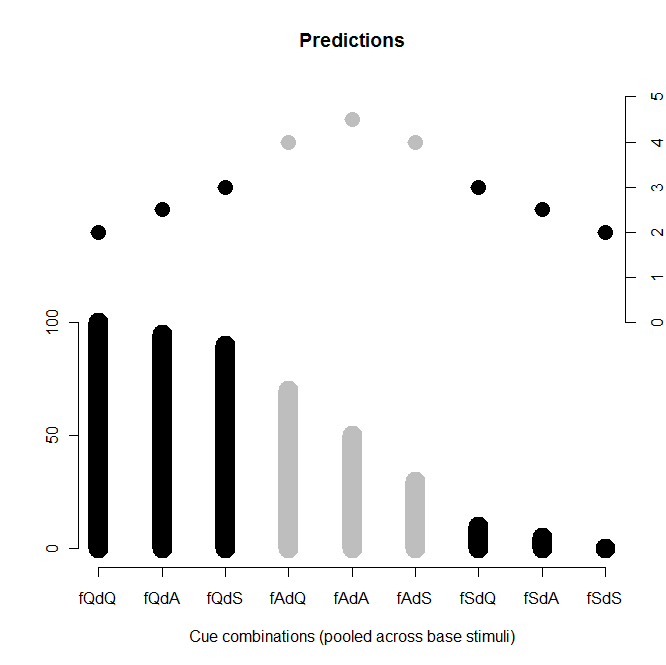
\includegraphics{images/501.png}}
\caption{Predicted question responses percent (bar plot) and reaction times (points) for the 9 resynthesis conditions: \textit{f} and \textit{d} indicate \textit{f0} contours and durational patterns, \textit{Q}, \textit{A} and \textit{S} indicate question-like, ambiguous and statement-like patterns.}
\label{fig501}\end{figure}
\subsection{Material}\label{sec522}
We used a resynthesis procedure partially based on work by \citet{gubian2010automatic,gubian2011joint} and implemented through a set of scripts in \textit{R} \citep{r2008r} and \textit{Praat} \citep{boersma2008praat}.\is{resynthesis} We extracted the segmentally aligned \textit{f0} contours of the two base stimuli (\textit{fQ, fS}) and turned them into continuous functions through b-spline smoothing. That is, the \textit{f0} curve was not discretized as is usually done in perceptual studies involving resynthesis. No top-down knowledge was fed into the resynthesis procedure, apart from anchoring the \textit{f0} contours to the segmental boundaries. Moreover, by using continuous phonetic representations instead of a sequence of turning points, we avoid losing potentially useful melodic information. Minimalist top-down based assumptions were also made in the extraction of the durational patterns of the two base stimuli (\textit{dQ, dS}), for which we stored the duration of each phone as annotated by manual segmentation.
Then we calculated an acoustically ambiguous durational pattern (\textit{dA}), by averaging phone durations, and an acoustically ambiguous \textit{f0} contour (\textit{fA}), by averaging functions with respect to the segmental landmarks. Function averaging was accomplished by extracting a transform function which turned a given contour into the opposite, and by applying it with a weight of 0.5. We resynthesized each of the two base stimuli with the nine combinations between the two factors (\textit{f} and \textit{d}) and their three levels (\textit{Q}, \textit{S} and \textit{A}), thus obtaining 18 experimental items.
\section{Results}\label{sec53}
A plot of the raw data shows that melodic cues alone are relevant in sentence modality contrasts perception.
As for identification results (Figure~\ref{fig502}), the strong effect of melodic manipulations is attested by the drop in question identification rates between stimuli with question intonation (\textit{bXfQdX}), with ambiguous intonation (\textit{bXfAdX})\footnote{For a discussion of the consistent bias toward question response in stimuli with ambiguous intonation, see Section~\ref{sec541}.} and with statement intonation (\textit{bXfSdX}). Temporal manipulations, on the other hand, do not seem to affect subjects' responses: none of the triplets above show an internal drop in question identification (e.g. given the triplet QX, same rates for QQ, QA and QS).
\begin{figure}
\centering
\resizebox{0.66\linewidth}{!}{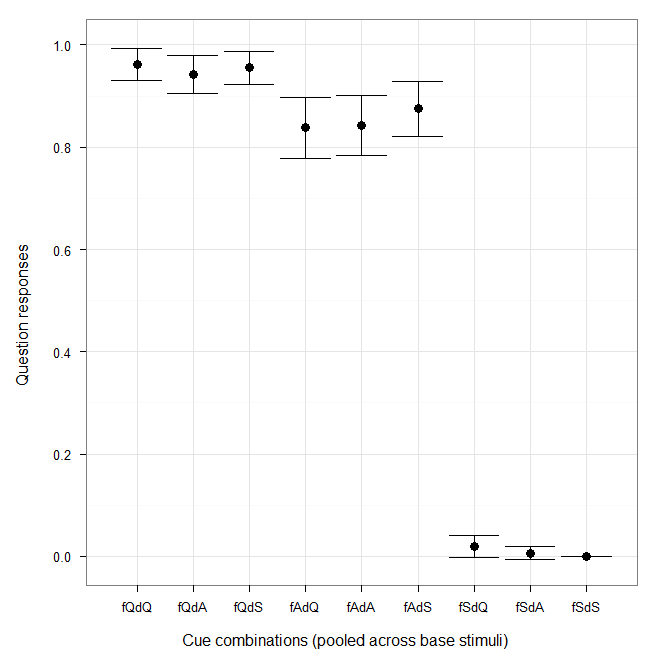
\includegraphics{images/502.png}}
\caption{Hypothesis 1. Observed question responses (mean and error bars) for the 9 resynthesis conditions.}
\label{fig502}\end{figure}
Reaction times also show no effect of temporal manipulations (Figure~\ref{fig503}). In particular, responses are not faster when stimuli have congruous (white) rather than incongruous (black) temporal and intonational cues. On the other hand, stimuli with ambiguous intonation elicited longer reaction times.
\begin{figure}
\centering
\resizebox{0.66\linewidth}{!}{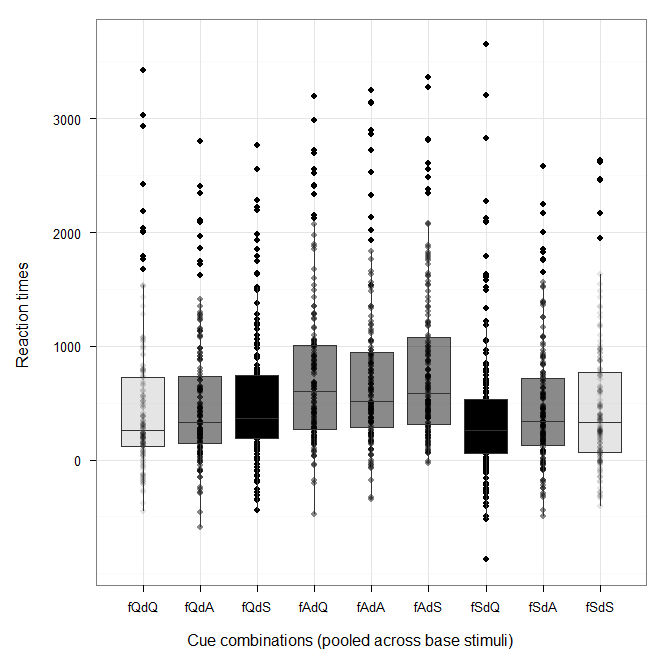
\includegraphics{images/503.png}}
\caption{Hypothesis 2. Observed reaction times (boxplot and observations) for the 9 resynthesis conditions. Congruous conditions in white, incongruous conditions in black (non relevant conditions in grey).}
\label{fig503}\end{figure}
\subsection{Orthogonality hypothesis}\label{sec531}
In order to test H1 we ran a series of generalized mixed logit models, aimed at evaluating the effect of temporal manipulations on subjects' identification responses. The most comprehensive model included the three fixed factors \textit{Intonation} (three levels: question, ambiguous and statement), \textit{Tempo} (question, ambiguous and statement), and \textit{Base} stimulus (question and statement), as well as their interaction, together with a random intercept for our 26 \textit{Subjects}. The model was then pruned, excluding three-way interactions first, then two-way interactions, and ultimately non-significant factors. As a result, the comparison between the most comprehensive model and the one containing the fixed factor \textit{Intonation} alone shows no significant Likelihood difference ($\chi^{2}=16.7, df=15, p=0.33$), thus leading to the rejection of H1.
\textit{A fortiori}, the corollary of a stronger effect of temporal manipulations for stimuli with ambiguous intonation is not validated either. The corollary would have been validated by significant interactions between \textit{Intonation} and \textit{Tempo}. However, as can be inferred from the comparison between the model including \textit{Intonation}, \textit{Tempo}, \textit{Base} and their interaction with the model containing \textit{Intonation} alone, no difference in Likelihood is attested when comparing the model containing \textit{Intonation}, \textit{Tempo} and their interactions with the model containing \textit{Intonation} and \textit{Tempo} alone ($\chi^{2}=5.6, df=4, p=0.23$).
\subsection{Nesting hypothesis}\label{sec532}
As for H2, we ran a series of generalized linear mixed models evaluating the effect of temporal manipulations on subjects' reaction times. Prior to modelling, latencies were made positive and log-transformed.\footnote{Since reaction times were calculated with respect to stimulus offset, a negative value for latency indicates that response to trial has been provided before the end of the stimulus itself. See Section~\ref{sec541} for discussion.} The most comprehensive model included the three fixed factors \textit{Intonation} (three levels: question, ambiguous and statement), \textit{Tempo} (question, ambiguous and statement), and \textit{Base} stimulus (question and statement), as well as their interaction, together with a random intercept for our 26 \textit{Subjects}. A Likelihood Ratio Test between this model and the one without the \textit{Base} factor showed no significant difference ($\chi^{2}=14.32, df=9, p=0.11$), so in the following we will only refer to the more economical model.
In our model, differences between response times to stimuli with congruous (\textit{bXfQdQ} and \textit{bXfSdS}) and incongruous (\textit{bXfSdQ} and \textit{bXfQdS}) sets of intonational and temporal cues are estimated by the interactions between intonation and tempo.\footnote{Specifically, if one takes latencies for \textit{bXfQdQ} as a reference (\textit{i}, intercept), one must estimate the coefficient for temporal manipulation from Question to Statement (\textit{tempoS}) in the case of \textit{bXfQdS}, the coefficient for intonational manipulation from Question to Statement (\textit{intonS}) in the case of \textit{bXfSdQ}, and the two previously mentioned coefficients along with the interaction between temporal and durational manipulations from Questions to Statement (\textit{tempoSintonS}) in the case of \textit{bXfSdS}. Grouping the four stimuli in the two congruous and incongruous conditions, we obtain that different latencies among the two groups require a significant coefficient for \textit{tempoSintonS}:
\begin{center}
$(bXfQdQ + bXfSdS) - (bXfSdQ + bXfQdS) =$\\
$= (i + i + intonS + tempoS + tempoSintonS) - (i + intonS + i + tempoS) =$\\
$= tempoSintonS$
\end{center}} A comparison between the model including \textit{Intonation}, \textit{Tempo} as well as their interactions with the model including \textit{Intonation} and \textit{Tempo} alone shows no significant Likelihood difference ($\chi^{2}=2.66, df=4, p=0.61$),\footnote{Specifically, the coefficient for \textit{tempoSintonS} is non significant ($t=0.11$).} thus leading to the rejection of H2.
\section{Discussion}\label{sec54}
Our results suggest that listeners do not use durational patterns as a cue for the identification of resynthesized stimuli as either questions or statements. Listeners' responses were not affected by resynthesis of temporal patterns, not even when intonational cues were made ambiguous. This finding speaks against a model of prosody in which tempo is seen as an orthogonal dimension to intonation, contra H1.
Moreover, identification of sentence modality does not seem to be hindered by a mismatch between melodic and temporal cues: reaction times were similar in responses to stimuli with either conflicting (i.e. \textit{bXfQdS} and \textit{bXfStQ}) or cooperating (i.e. \textit{bXfQdQ} and \textit{bXfSdS}) cues. In these cases as well, listeners only seemed to rely on intonation. This finding is not consistent with the hypothesis that temporal information is part of representations for intonational categories, contra H2 as well. Response times are only slightly higher when intonation is made ambiguous, a fact which can be seen as additional evidence for the exclusive role of intonational cues.
In sum, it seems that temporal detail is not a cue to the perception of sentence modality contrasts.
\subsection{Design-related issues}\label{sec541}
Before discussing the epistemological issues which limit the scope of our findings (Section~\ref{sec542}) and concluding on their possible relevance in the broader frame of research on prosodic detail (Section~\ref{sec55}), we now turn to an examination of some issues in the experimental design which could have affected our results, and report on a small-scale spin-off experiment which addressed part of them.
\subsubsection{Resynthesis}\label{sec5411}\is{resynthesis}
Experimental stimuli were created with an innovative resynthesis procedure, which combines modifications of \textit{f0} contours and of temporal patterns (see Section~\ref{sec522}). Since the procedure was elaborated for the purposes of this study, no independent testing of its performance was available. However, in addition to being used for the evaluation of our research hypotheses on tempo, the data collected for our experiment can also be used to provide a first evaluation of the continuous resynthesis of \textit{f0} contours.
Subjects' responses show that cross-modality manipulation was extremely successful. Identification responses were not affected by the nature of the stimulus used as base for the resynthesis: question identification for natural questions (\textit{bQfQdX}) and for natural statements resynthesized with question intonation (\textit{bSfQdX}) is not significantly different, and the same holds for question to statement resynthesis.\footnote{In the Generalized Mixed Logit model predicting subjects' responses from \textit{Intonation} and \textit{Base} as fixed factors, together with their interactions and adding a random intercept for \textit{Subjects}, no base-related coefficient reaches the significance level. Excluding the \textit{Base:Intonation} interaction for stimuli with ambiguous intonation (which are not relevant for the present discussion, and in any case non significant as well: $\beta=0.98, z=1.70, p=0.09$), \textit{Base} ($\beta=-0.45, z=-0.93, p=0.35$) and \textit{Base:Intonation} interaction ($\beta=0.45, z=0.35, p=0.72$) fail to reach significance.}
On the other hand, the resynthesis procedure could not produce a truly \textit{perceptually ambiguous} \textit{f0} contour between questions and statements. Stimuli intended to be intonationally ambiguous (\textit{bXfAtX}) were identified as question well above chance level (see Figure~\ref{fig502}). This finding is not surprising. As we said above (see Section~\ref{sec522}), ambiguous contours were obtained by setting to 0.5 the transformation coefficient \textit{c} or, in other words, by calculating the arithmetic mean of the two time-warped \textit{f0} contours. In order to achieve truly ambiguous stimuli with a procedure of this kind, the perceptual space between questions and statements should be linear. However, the non-linear warping of perceptual space has been long acknowledged for contrasts at the segmental level, which makes the assumption of a linear perceptual space for utterance-wide intonational contrasts even more untenable \citep{gubian2010automatic}. By allowing a fine-grained control of separate acoustic dimensions, our resynthesis procedure is indeed especially suited for the exploration of the perceptual space of intonational contrasts, which would ultimately provide the necessary insights for the creation of truly perceptually ambiguous stimuli. In the absence of this preparatory work, for the purposes of our current study we consciously restrained to the simplistic choice of using \textit{acoustically ambiguous} stimuli.
It has to be noted, however, that the use of acoustically rather than perceptually ambiguous stimuli potentially hinders the complete evaluation of H1 (\textit{orthogonality} hypothesis). As we said above, in the hypothesis of an independent processing of temporal and melodic cues, we made the corollary prediction that the effect of temporal manipulations is stronger if melodic information is made ambiguous or unavailable. The fact that our resynthesis procedure only yielded stimuli with acoustically (and not perceptually) ambiguous melodic information does not allow us to draw definitive conclusions on this prediction. However, discarding the main hypothesis of significant temporal-related effects across all stimuli entails discarding the corollary prediction of stronger temporal-related effects when no intonational cues are available. This does not mean that proper resynthesis of perceptually ambiguous intonation is unnecessary in the evaluation of temporal effects. We could also formulate a separate hypothesis, stating that temporal-related effects are significant \textit{only} when no intonational cues are available. In this case, our data on exclusively acoustically ambiguous stimuli would not be conclusive.
\subsubsection{Reaction times}\label{sec5412}
As we said above (see Section~\ref{sec512}), the evaluation of H2 as well needs particular caution. We suggested that the relevance of temporal information in the phonological representations of intonational contrasts (\textit{nesting} hypothesis) could have been indicated by different reaction times between stimuli with congruous (\textit{bXfQdQ} and \textit{bXfSdS}) and incongruous (\textit{bXfSdQ} and \textit{bXfSdQ}) information on the melodic and temporal levels. However, the quantitative evaluation of significant differences in reaction times is affected by two kinds of issues.
On a lower level, a first problem is represented by the fact that total stimulus duration was not fixed. The production experiments in Section~\ref{sec4} showed that global utterance duration is not significantly different across questions and statements. However, this does not mean that differences in the duration of individual items are unattested. Specifically, the durations of the utterances used as bases for the resynthesis procedure were 1.2 sec for the statement version (\textit{bXfXdS}) and 1.3 sec for the question (\textit{bXfXdQ}). Since resynthesis of ambiguous durational patterns was based on arithmetical averaging (see discussion in the subsection above), duration of temporally ambiguous stimuli was 1.25 sec (\textit{bXfXdA}). Given that \textit{Perceval} calculates reaction times with reference to stimulus onset, stimulus duration was subtracted from latencies in order to obtain results which can be interpreted as reaction times from the end of the stimulus.
However, given the nature of our stimuli, can we really consider reaction times as a reliable measure for the validation of H2? Response latencies from stimulus offset would be an indicator of ease of processing only if listeners delayed the evaluation of (mis)match between melodic and temporal information until the end of stimulus. This, however, is only a simplifying assumption, made in the absence of relevant knowledge on the integration of suprasegmental cues in perception of post-lexical meaning. Indeed, there is reason to believe that, since temporal and melodic cues unfold in time, their integration could be best captured by on-line tasks or by the monitoring of multiple references for reaction times. Specifically, as for intonation, the very idea of analyzing phonetic data (\textit{f0} contours) as a succession of phonological events (pitch accents and edge tones) entails the existence of multiple points in time where bundles of perceptually relevant material is made available. If we chose to measure reaction times from utterance end, it is because the experiments of Section~\ref{sec4} showed that durational patterns are best characterized as variations of speech rate across the utterance. However, future studies on the interplay between temporal and melodic cues should definitely take into account the possibility of evaluating cue integration as time unfolds.
As for the more restricted purposes of our study, the use of response latencies relative to utterance end is a factor which could have limited the conclusiveness of H2 validation. In particular, in the case of attested statistically significant difference between reaction times to congruous and incongruous stimuli, the evaluation of its perceptual meaningfulness would have required further research. However, since our data show that no significant differences are attested, H2 can be safely rejected.
\subsubsection{Spin-off}\label{sec5413}
As we said above, if we assume that tempo is a secondary cue to sentence modality, a corollary of the orthogonality hypothesis (H1) is that differences in durational patterns are best perceived when intonational cues are not available. That is, we expect a greater difference between responses to stimuli with question-like and statement-like durational patterns for items with ambiguous \textit{f0} contours than for items with either question-like or statement-like \textit{f0} contour. This motivates the steeper fall in the hypothesized rate of question responses for the grey triplet in Figure~\ref{fig501}, compared to the black triplets. That is, maximal difference in subjects' responses is expected between the pairs \textit{bXfAdQ} and \textit{bXfAdS}.
Our results did not support the orthogonality hypothesis (see Section~\ref{sec53}). Moreover, resynthesis of ambiguous \textit{f0} contours was not entirely satisfactory. However, given the set of stimuli used in the task, we cannot rule out the possibility of ceiling effects in subjects' responses due to the availability of intonationally unambiguous stimuli. That is, listeners' attention might have been diverted from subtle temporal cues because of the presence of striking intonational differences. For this reason, we devised a short spin-off experiment to be ran after the main test. Subjects were asked to identify as question or statements stimuli in the \textit{bXfAdQ} and \textit{bXfAdS} conditions alone; no fillers or intonationally clear stimuli were presented. We hypothesized that, if durational differences are perceptible and used in sentence modality categorization, presenting intonationally ambiguous stimuli \textit{alone} would have maximised the visibility of the effect of tempo on perception.
We gathered responses from 26 subjects for the 2 conditions resynthesized from 2 bases, presented 4 times in each of 2 independently randomized blocks, for a total of 832 items. Subjects' \textit{Responses} were predicted using a generalized linear mixed model with \textit{Tempo} as a fixed factor and \textit{Subject} as a random factor. The coefficient for Tempo, however, did not prove significant ($\beta=-0.03, z=-0.199, p=0.843$). This shows that, even when stimuli are presented such as to maximize listeners' attention to temporal manipulations, durational differences are not a cue to sentence modality contrasts.
\subsection{Epistemological issues}\label{sec542}
The main limitation to the use of our results in drawing clear-cut conclusions on the role of tempo as a prosodic detail, however, comes from a different source. Our experiment aimed at evaluating whether the acoustic differences in durational patterns we documented with our production study (see Sections~\ref{sec43} and~\ref{sec44}) are used as a cue in the perception of sentence modality contrasts. A positive answer to this research question would have implied that tempo has to be somehow included in phonological representations of intonation (H2) or prosody (H1). The negative evidence (H0) we gathered through our experiment, on the other hand, does not allow us to draw the opposite conclusion, namely that tempo should \textit{not} be included in phonological representations.\is{good effort} The scope of generalization for negative findings must be accurately determined. We can only state that perception of \textit{sentence modality} contrasts in NI clean read speech is not affected by durational differences, but we cannot rule out that durational differences play a role in the perception of other linguistically structured contrasts or in other communicative contexts.
To be more specific, the scope of our results can be further narrowed down to the conclusion that perception of sentence modality contrasts is not affected by durational differences \textit{as we modelled them} in Section~\ref{sec4}, and namely as related to variations in phone durations (rather than lower or higher level units). We cannot exclude that, had we modelled production differences in a different way, perceptual evaluation could have yielded positive results. The production study presented in Section~\ref{sec43} might have been, at the same time, a starting point and a bottleneck to our perceptual validation. Before definitively dismissing the hypothesis of a perceptual relevance for temporal detail, further explorations of its acoustic manifestation could be necessary.
Pushing this line of reasoning to its extremes, the scope of our testing cannot actually be stretched beyond the role of phone durations in cueing sentence modality contrasts for our \textit{two base stimuli}. The input for our resynthesis procedure consisted in \textit{f0} contours and durational patterns extracted from two individual utterances, which were (transformed and) combined to yield nine test stimuli. Thus, in a radical perspective, we cannot exclude that choosing a different pair of base stimuli could have affected our results as well.
On the other hand, in the view of our discussion above on production modelling as a bottleneck to perceptual validation, the use of a data-driven resynthesis procedure based on the properties of individual stimuli (rather than on an explicit rule-based modelling of the allegedly relevant dimensions) could also prove an effective choice. In a data-driven approach to resynthesis, in fact, there is less room for top-down fed information, and thus the downfalls of an incorrect modelling of production data are strongly limited. For example, our intonational resynthesis gave excellent results (see Section~\ref{sec541}) by simply warping time-aligned \textit{f0} contours. In other words, all previous knowledge from the literature on the phonetics and phonology of intonation was condensed and limited to ``alignment of \textit{f0} contours with segmental boundaries is relevant''. For cross-modality resynthesis of utterances with the same segmental content, this top-down information alone caused a 94\% shift\footnote{This is the absolute value of the estimated coefficient of question to statement manipulation in a linear mixed model predicting subjects' \textit{Response} (coded as a continuous variable) from \textit{Intonation} as a fixed factor and \textit{Subject} as a random factor. The coefficient was highly significant ($t=62.53$).} in subjects' identification responses. For temporal resynthesis, we limited our assumptions to ``variations in segmental durations are relevant'', as the most general formulation of the findings from our production study.\footnote{The segmental level was preferred over smaller (i.e. subsegmental phases) or bigger (e.g. syllables) domains, as a reasonable compromise between a fine-grained temporal analysis and the degree of precision allowed by our forced alignment tool (see Section~\ref{sec422}).} That is, as in the case of intonation above, we did not feed the procedure with specific information from our own account of temporal differences across sentence modality. Our interpretation of the role of the edge segments in the utterance (see Section~\ref{sec434}) or of the interaction between modality and focus (see Section~\ref{sec444}) does not inform the resynthesis procedure we used in this chapter: rejection of our account of produced temporal detail (Section~\ref{sec4}) does not entail rejection of the perceptual validation we provided here.
In sum, as in the case of every study in which the alternative hypotheses are not supported, no definitive statement can be inferred from our results. We have to limit the scope of our conclusions according to the features of our study, and restrain from claiming that temporal detail is irrelevant in cueing post-lexical meaning. We can nonetheless conclude that its effects are hard to track in sentence modality contrasts in read speech, that its exploration is unlikely to reveal the need for an enrichment of the phonological structure of prosody, and that its perceptual evaluation is ultimately a sorely unrewarding enterprise.
\section{Conclusion}\label{sec55}
In this chapter we tested the perceptual role of different durational patterns in sentence modality contrasts. The experiments in Section~\ref{sec4} showed that production of questions and statements in Neapolitan Italian is characterized by subtle but consistent differences in segmental durations. However, these acoustic differences do not seem to be used as perceptual cues: listeners' responses in a forced choice identification task are not affected by the manipulation of durational patterns. Moreover, no difference was found in response times to stimuli with congruous and incongruous information on the temporal and on the melodic levels. These findings are consistent with an abstractionist view of perception of post-lexical contrasts, in which some of the available information on regularly produced contrasts is indeed discarded.
However, both methodological and epistemological issues prevent us from considering the evidence gathered in this chapter as truly conclusive. On the one side, the multiparametric resynthesis procedure used in the creation of the experimental stimuli should be refined, especially as far as the creation of intonationally ambiguous stimuli is concerned. Our procedure performs nonetheless very well in cross-modal resynthesis of intonation, and could represent a useful tool in the exploration of perceptual space at the utterance level. On the epistemological side, since the experiment was designed to test the perceptual importance of temporal detail, we only found evidence supporting the null hypothesis, a fact which limits the scope on the generalizability of our findings.
With these caveat in mind, we can still conclude that, inside the limited scope of our investigations, temporal detail in NI does not appear to be as salient as the melodic detail we explored in Sections~\ref{sec2}--~\ref{sec3}. The findings of Section~\ref{sec4}, while tapping into relationships between phonetic cues which are potentially interesting in the study of production mechanisms, cannot be stretched to constitute evidence for the existence of meaningful prosodic detail at the temporal level. In conclusion, we have reason to believe that an expansion of our phonological accounts of prosody with the inclusion of the temporal dimension can be safely postponed until more compelling evidence is gathered.
